% \subsection{Enterprise Structure}
Large enterprises have traditionally implemented formal, centralized forms of organizational structure~\cite{pearlson2009}, such as hierarchical or matrix structures. In these structures, communication patterns, roles and decision rights are strictly defined. This allows for management to have a high degree of control over the enterprise and therefore enforce compliance with standards, procedures and policies which results in a highly stable enterprise. However, this comes at the expense of agility; it is difficult for these organizations to quickly adapt to a changing environment. While centralized structures were appropriate for the business environments of the past, modern business environments demand a high level of agility.

Common components of modern business environments include cooperation with different organizations,  rapidly changing business activities and processes, and a rapidly changing competitive landscape. In order to properly handle these components, a high level of enterprise agility is necessary. In centralized organizations, decisions need to be discussed at all levels of the hierarchy in order to obtain the appropriate justification and approval. This takes time; by the time a decision is made, it is often too late for it to be effective. In contrast, having decision making on the operational level allows for quick decisions that enables an organization to take advantage of opportunities quickly. More decentralized structures, such as networked organizations~\cite{pearlson2009}, are examples of this. It is important to note that a lack of rigidity and formal structure does not mean a lack of organization. It is still important for a decentralized enterprise to maintain order in its activities; this organization just needs to be based on an underlying decentralized structure instead of centralized one. Consequently, decentralized organizations need solutions to the same problems faced by centralized organizations -- such as business-IT alignment -- but the solutions need to be supportive of decentralization over centralization. 

Decentralization and agility in organizations needs to be supported by IS. IS architectures exist that can support decentralization, for example Service-Oriented Architecture (SOA), but organizations need to use them to implement IS that is supportive of the organization. This issue of alignment between business and IT is one that is addressed by the practice of Enterprise Architecture (EA). 

Enterprise Architecture is a practice for creating an architecture for an entire enterprise or organization. EA takes a holistic view of an enterprise in order to bring its many components -- such as goals, strategies, information systems, processes, and governance styles -- into alignment with each other. Many different EA frameworks currently exist, for example The Open Group Architecture Framework (TOGAF)~\cite{togaf9.1}, the Zachman Framework~\cite{zachman} and Federal Enterprise Architecture (FEA)~\cite{FEA_PMO2007}. 

All frameworks address one or more of the following three different aspects: artifacts that describe an enterprise's architecture, the process of creating these artifacts, and a way to ensure that the architecture implementation is an ongoing success. In this thesis, these three elements are respectively referred to as the EA description, EA method, and EA engine (Fig~\ref{fig:EA_general}). 

By creating an architecture for all components of an enterprise, EA is a solution to the problem of business-IT alignment. Therefore, in this thesis we analyze modern EA frameworks for their support of decentralization in organizations. Support for decentralization in EA frameworks would allow for EA to be a solution for business-IT alignment in decentralized organizations. 

\begin{figure}
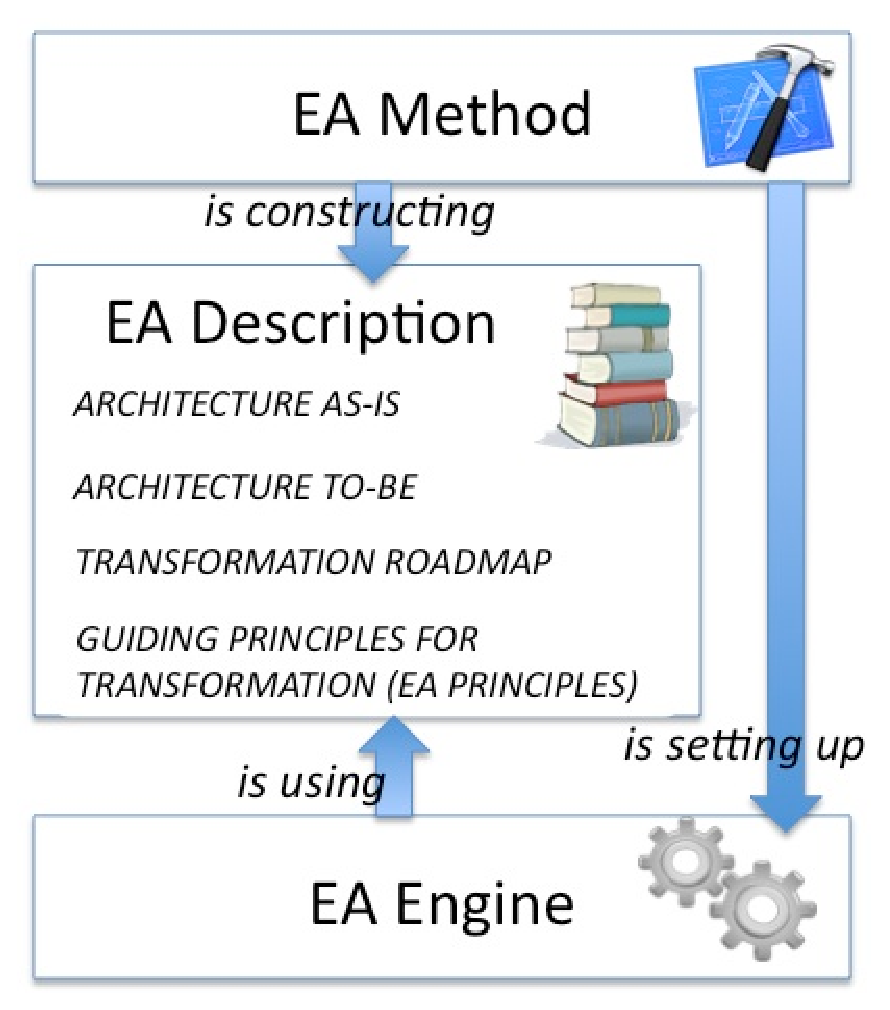
\includegraphics[scale=0.5]{EA}
\caption{Enterprise Architecture}
\label{fig:EA_general}
\end{figure}

%Enterprises are not alone in their trend towards decentralization; this trend also exists elsewhere. For example, peer-to-peer architectures -- where peers communication directly to each other, without the need for a central server -- are becoming increasingly popular.  These architectures now exist in many different areas, such as file sharing~\cite{bittorrent}, content distribution~\cite{blizzard}, revision control~\cite{progit}, as a digital currency~\cite{bitcoin2008}, for the funding of creative projects~\cite{kickstarter}, for moderation~\cite{reddit, slashdot}, and for content creation~\cite{wikipedia}. As a result, this thesis will look to take principles from peer-to-peer architectures and apply them to EA for increasing their support of decentralization. 


